\chapter{\color{oxfordblue} The ATLAS Experiment and the LHC}\label{chapter-ATLAS}
\ChapFrame

\textit{
Modern particle physics is at the edge of the technological reach of science. To discover the Higgs boson, an extremely complex infrastuctre is required to probe physics at the required scale. The \gls{lhc} at \gls{cern} is consequently the largest and most powerful particle accelerator and has held this title since its construction in 2008 \cite{LyndonEvans_2008}. It is easily ranks as one of the mox complex machine ever created. Protons are accelerated to up to 99.9999991\% of the speed of light, in a giant 27 km long ring-shaped accelerator, burried 100 m below the surface of the French-Swiss border near Geneva. Superconducting magnets cooled down with liquid helium to 1.9 $K$ steer steer this an energetic beam thanks to powerful magnetic fields of 8.33 Tesla. The beams are made of bunches of particles, collided precisely at four specific interactions points where large detectors are built and operated by dedicated experiments: ATLAS \cite{TheATLASCollaboration_2008}, CMS \cite{TheCMSCollaboration_2008}, ALICE \cite{TheALICECollaboration_2008}, and LHCb \cite{TheLHCbCollaboration_2008}. The first two are multi-purpose experiments with overlapping physics programs, while ALICE and LHCb are respectively dedicated to heavy ion and heavy flavour physics. This chapter described the experimental setup of the \gls{lhc} and the ATLAS experiment, focusing on proton-proton collisions and introducing relevant elements to the work presented in this thesis.} 

\section{The Large Hadron Collider}\label{sec-LHC} % TODO check values

\begin{figure}[!h]
  \centering
  \makebox[\textwidth][c]{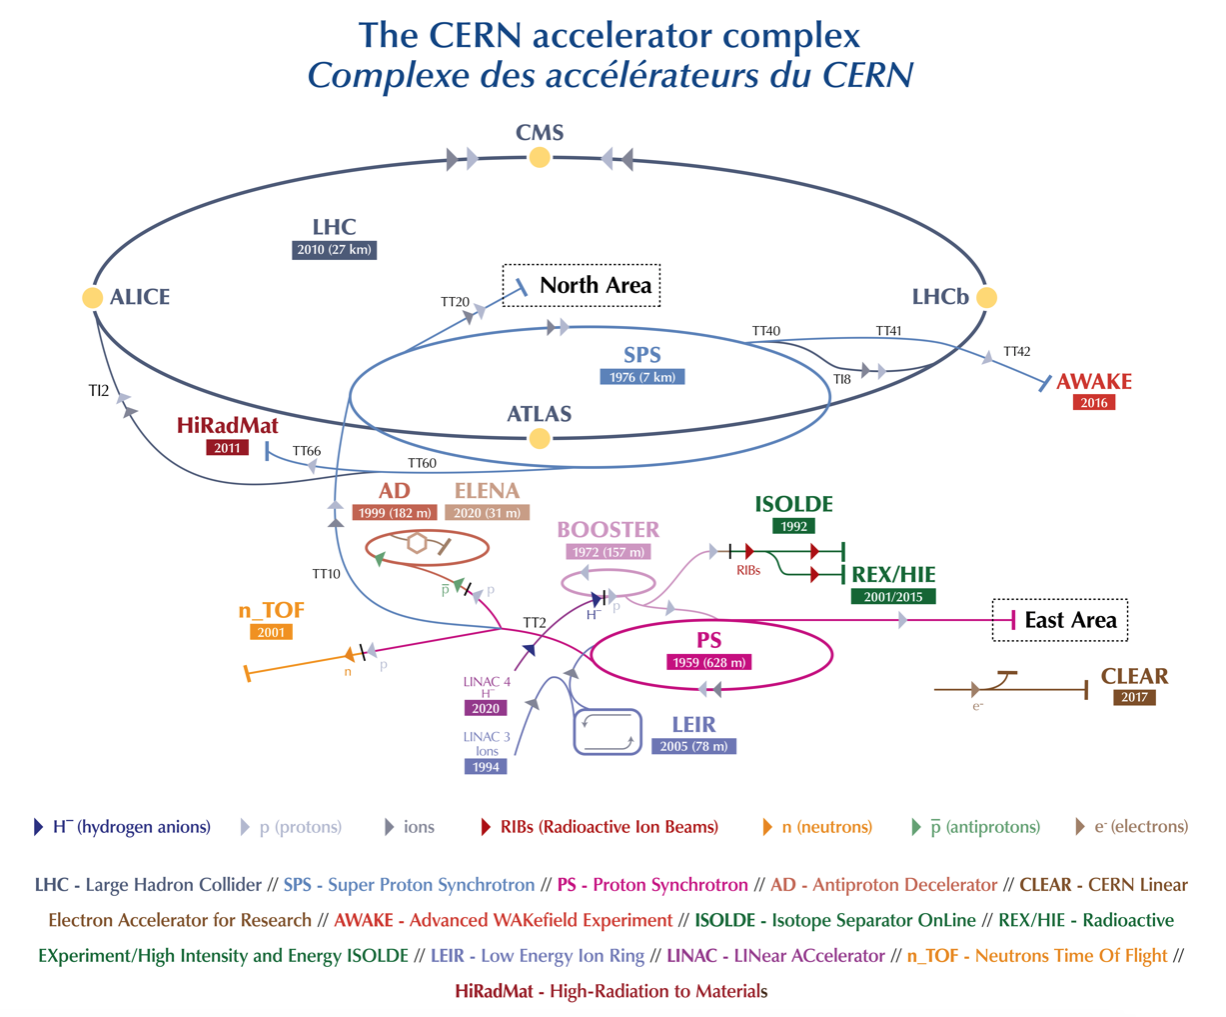
\includegraphics[width=1.05\textwidth]{Images/ATLAS/cernAcc}}
  \caption{The accelerator complex of CERN during Run 2 \cite{CERNAcc}. The LHC is the top dark blue ring.}
  \label{fig-CernAccSys}
\end{figure}

The last machine in a complex multi-stage accelerator complex of CERN displayed in Figure \ref{fig-CernAccSys}, the \gls{lhc} is capable of frontally colliding proton or heavy ion beams. These beams are made of bunches of particles, collided precisely at four interactions points where large detectors are built and operated by dedicated experiments. The life of a proton beam starts innocuously ionised hydrogen $H^-$ gas, passed to a linear accelerator called LINAC4\footnote{Before 2020, it was LINAC2.} to reach energies of 160 MeV. After stripping the ionised hydrogen of its two electrons thus leaving a bare proton, the next acceleration stage is in the Proton Synchroton Booster (BOOSTER) bringing the beam energy to 2 GeV. The protons are then passed to increasingly larger synchrotons: the Proton Synchrotron (PS) to reach energies of 26 GeV, followed by the Super Proton Synchrotron (SPS) to reach energies of 450 GeV. The beam is finally injected into the \gls{lhc} in two different beamlines circulating the proton in opposite directions. Superconducting dipole magnets reaching 8.33 T steer the highly-energetic beams, while complex geometries of magnets (quadrupoles, sextupoles, ...) are deployed to refine the bunch shape through focusing effects. Powerful radiofrequency cavities accelerate them to their final energy of to 6.5 TeV, giving a total $pp$ centre of mass energy of $\sqrt{s} = 13$ TeV in Run 2.  \\

The operation of the \gls{lhc} is split into dedicated \textit{runs} of data taking, separated by \textit{shutdowns} to maintain or upgrade the infrastucture. Some key metrics from these runs from the point of view of the ATLAS experiment are displayed in Table~\ref{tbl:LHCATLASperf}
\begin{table}[!htbp]
    \begin{center}
        \renewcommand{\arraystretch}{1.2}
      %\resizebox{0.99\textwidth}{!}{
        \begin{tabular}{cc|cccc} \hline \hline 
          & Year & $\sqrt{s}$ [TeV] & $\langle \mu \rangle$ &  Luminosity $\mathcal{L}$ [cm$^{-2}$s$^{-1}$] & $\int\mathcal{L}$ [fb$^{-1}$] \\ \hline
          Run 1 & 2010 - 2012 & 7-8    & 18 & 0.8 $\times$ $10^{34}$    & $26.4$ \\
          Run 2 & 2015 - 2018 & 13     & 34 & 1-2 $\times$ $10^{34}$  & $140.1$ \\
          Run 3 & 2022 - 2025 & 13.6     & 50 & 2 $\times$ $10^{33}$    & $65$ \\

          \hline\hline
        \end{tabular}
      %}
      \caption{Metrics on the accerelarator performance of the LHC in the different runs of data taking. The reported values correspond to those recorded by the ATLAS experiment \cite{ATLAS:run1Lumi, ATLAS:2022hro, ATL-DAPR-PUB-2023-001}. Numbers for the ongoing Run 3 are preliminary, with the integrated luminosity listed considering events recorded until July 2023. The number of interactions per bunch crossing averaged over each run is displayed as $\langle \mu \rangle$.} % TODO Define BL and d0
      \label{tbl:LHCATLASperf}
    \end{center}
\end{table}

Run 2 operated at a larger centre of mass energy ($\sqrt{s}$) and higher average instantaneous luminosity $\mathcal{L}$ than Run 1, with Run 3 again pushing up the limits. The average instantaneous luminosity measures the quantity of data collected from the relation
\begin{equation}
  \mathcal{L} = \frac{1}{\sigma}\frac{dN}{dt}
\end{equation}
relating the event rate of a particular process to its cross-section $\sigma$. The instantaneous luminosity is a machine parameter: it depends on the design and the operation of the accelerator. It is calculated from
\begin{equation}
  \mathcal{L} = \frac{N_1N_2N_bf}{4\pi\sigma_x\sigma_y}
\end{equation}
where $N_1$ and $N_2$ are the number of protons in each bunch, $N_b$ the number of bunches, $f$ is the collider revolution frequency, and $\sigma_x$ and $\sigma_y$ are the $x$ and $y$ geometrical extension of the beam density distributions. The integrated luminosity $\int \mathcal{L} dt$ is a direct measure of the quantity of data collected over a certain period, often expressed in units of inverse \textit{barn} b$^{-1}$, where b $= 10^{-28}$ m$^{2}$. For Run 2, the total luminosity recorded corresponds to 140.1 $\pm$ 1.2 fb$^{-1}$, with a small uncertainty of 0.83 \% \cite{ATLAS:2022hro} thanks to a complex measurement involving luminosity-dedicated detectors such as LUCID-2 \cite{Avoni_2018}. Figure \ref{fig-atlasLumiPileup} shows the cumulative total integrated luminosity during Run 2, jointly with another important machine parameter: the average number of interactions per bunch crossing $\langle \mu\rangle$. 

\begin{figure}[!h]
  \centering
  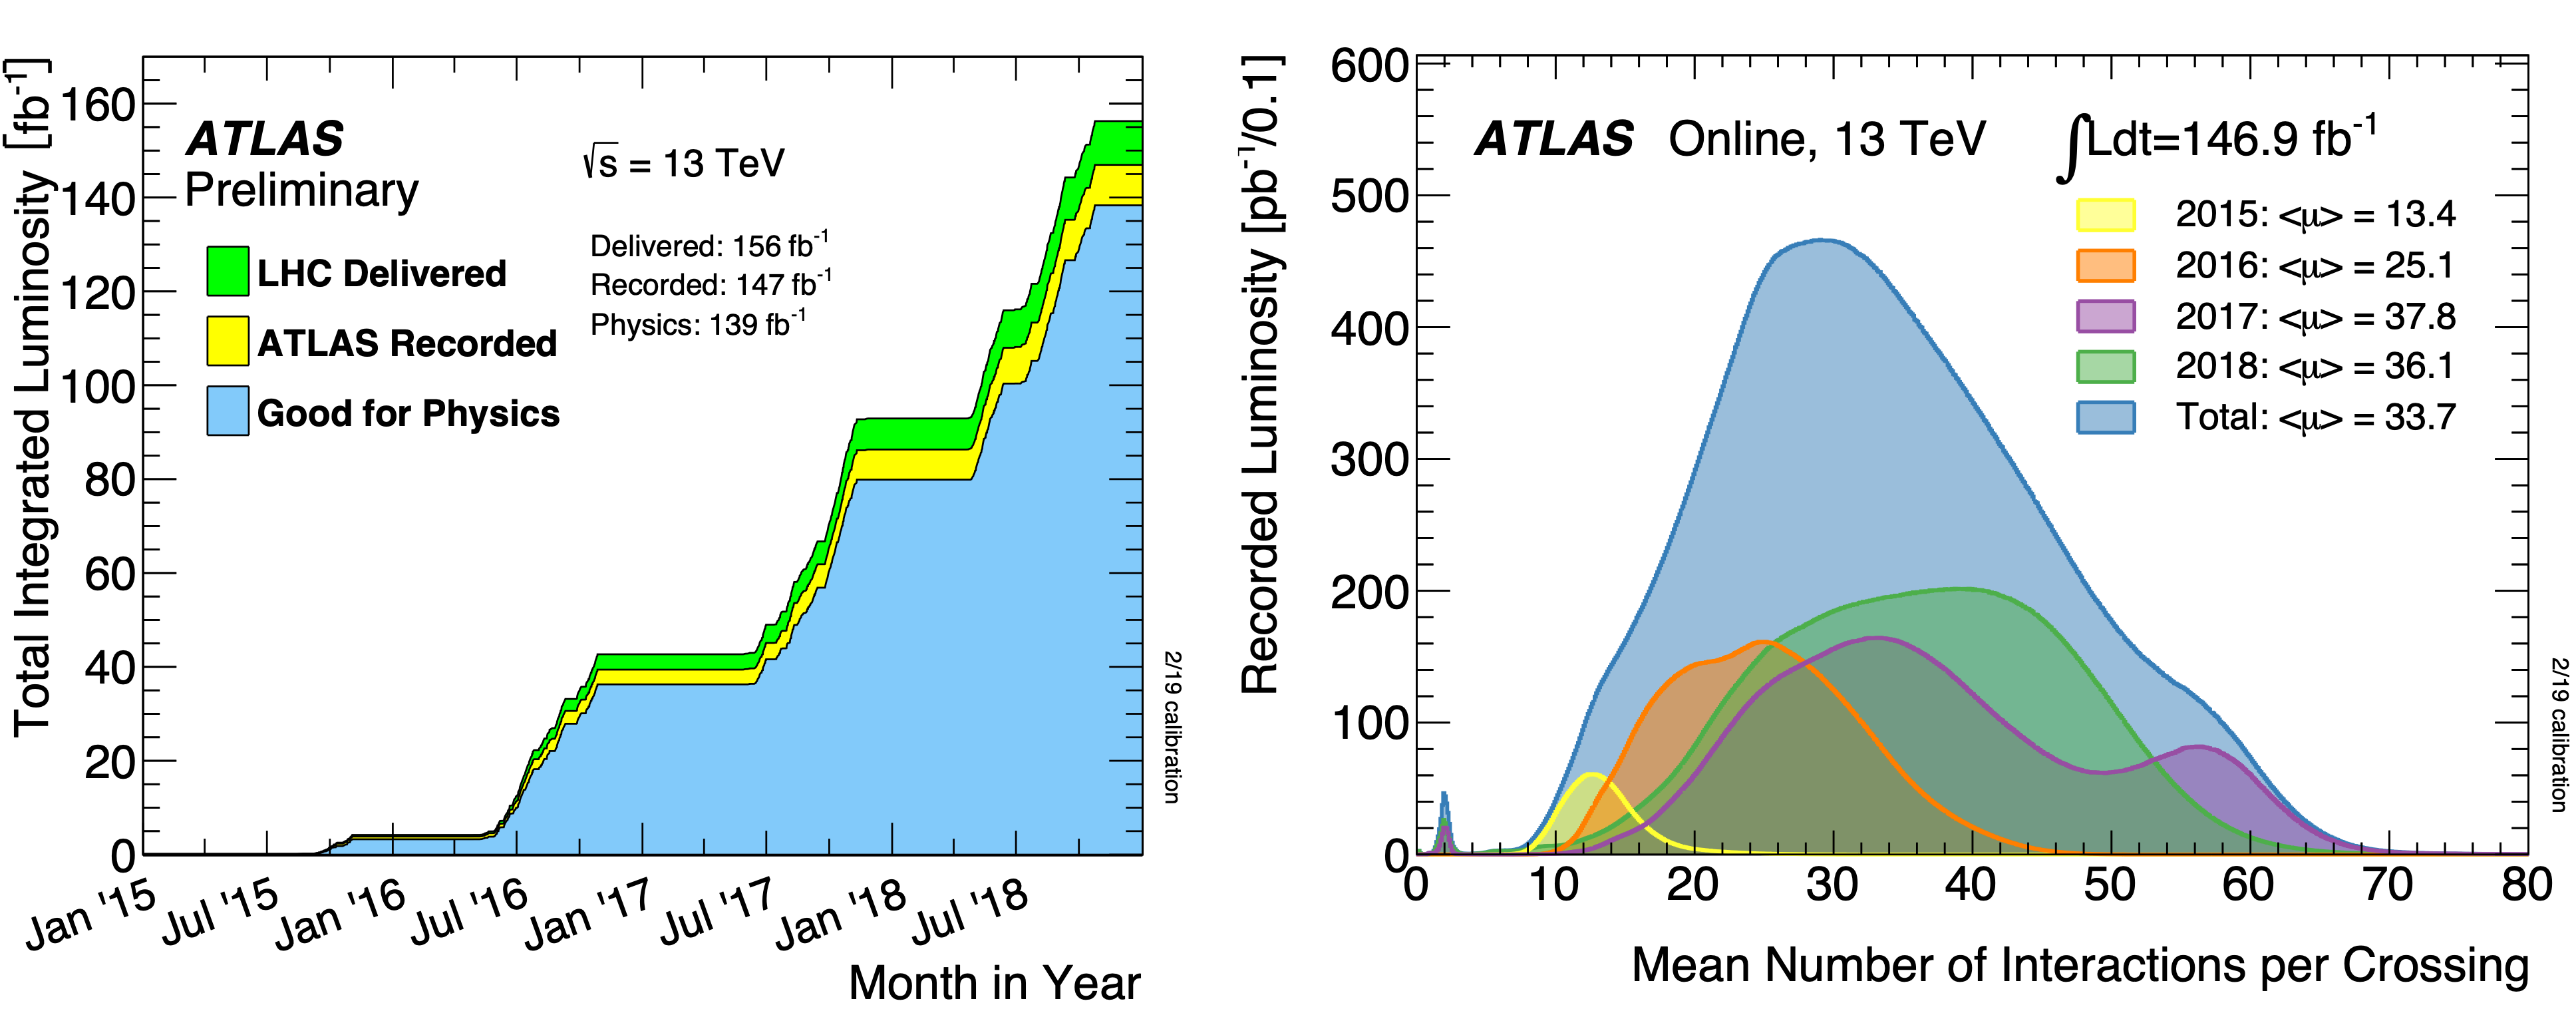
\includegraphics[width=\textwidth]{Images/ATLAS/recoATLAS.png}
  \caption{The ATLAS cumulative integrated luminosity delivered, recorded, and approved for physics (left) and the average pile-up distribution weighted by luminosity (right) during Run 2  \cite{PubAtlasLumi}. The luminosities indicated correspond to an early calculation that was corrected in Ref. \cite{ATLAS:2022hro}.}
  \label{fig-atlasLumiPileup}
\end{figure}

The main event during the collision of the proton bunches is the hard scatter where most of the energy transfer occurs. Other protons in the bunches do have softer interactions leading to background activity called \textit{\gls{pu}}. Two types of pile-up are distinguished: \textit{in-time \gls{pu}} when the soft interaction is from protons in the same bunch as the hard scatter recorded, and \textit{out-of-time \gls{pu}} when the protons are from another bunch crossing. Bunches in the \gls{lhc} are separated by a 25 ns delay, corresponding to a machine frequency of 4000 MHz. To control the luminosity, the angle of attack of the beams can be tweaked so that their overlap on the impact point is modified. Having more frontal collisions leads to a larger overlap and  a higher luminosity at the price of more \gls{pu}. 

\section{The ATLAS Detector}\label{sec-ATLASDet}
The ATLAS Collaboration built and operates the eponymous cylindrically shaped multi-layered detector lying 100 m underground with a length of 45 long and a 26 m diameter \cite{TheATLASCollaboration_2008}, as presented in figure \ref{AtlasDec}. The experiment is constructed to probe a braod range of physical phenomena, as required from the general purpose of the Collaboration. Aiming to be as hermetic as possible, the detector wraps around the interaction point with the barrel forming the central part of the cylinder and the end-caps closing the geometry at its extremity. Essential characteristics of the design had to be met to manage the extremely high event rate, requiring fast response, radiation-hard sensors, and state-of-the-art readout electronics in combination with good spatial and temporal resolution to disentangle the effect of pile-up. 

\begin{figure}[!h]
\centering
\hspace{-1.25cm}
\makebox[\textwidth][c]{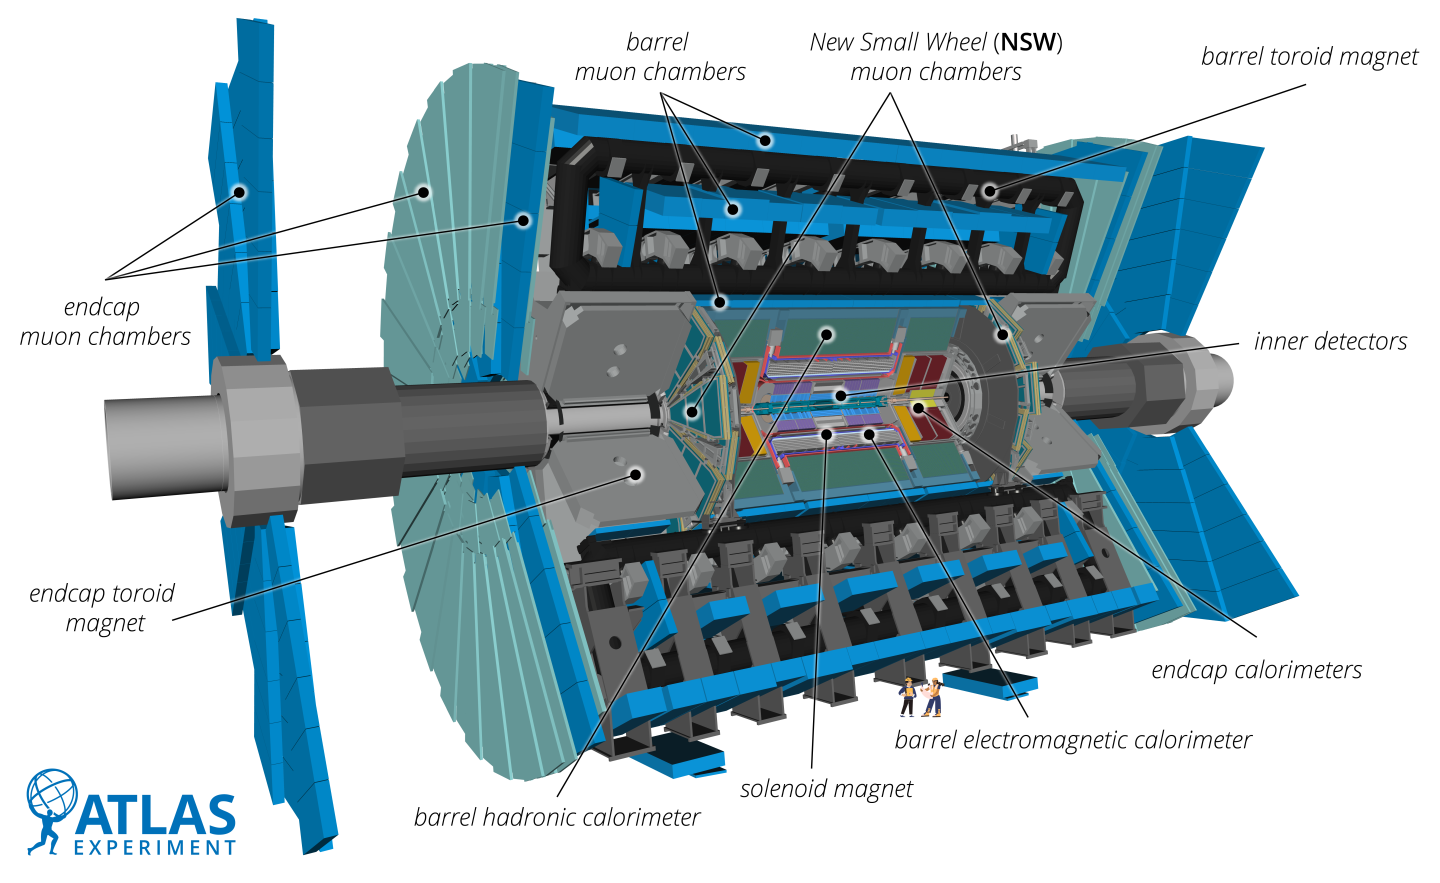
\includegraphics[width=1.08\textwidth]{Images/ATLAS/atlasDet.png}}
\caption{Cut-away view of the ATLAS detector \cite{ATLASschematics}.}
\label{fig-AtlasDec}
\end{figure}

The coordinate system adopted in ATLAS is described in Figure \ref{fig-AtlasCoord}: the $x$-axis point to the centre of the \gls{lhc} ring, the $y$-axis point upwards, and the $z$-axis in the direction of the beamline (anti-clockwise from the top). The azimuthal angle $\phi$ is defined in the transverse plane $x-y$ and the polar angle $\theta$ is measured upwards from the beam-axis (along $y$). Therefore, the transverse momentum \pt\ of a particle is obtained from its momentum vector $\boldsymbol{p} = (p_x, p_y, p_z)$ as: \pt\ $=\boldsymbol{p} \sin\theta = \sqrt{p_x^2 + p_y^2}$. This is of particular interest as the momentum's longitudinal component $p_z$ is not measurable due to the openings for the beamline and the partonic interaction carrying only a fraction of the original proton momentum. Only the transverse momentum can be correctly assessed, as the initial parton is mostly boosted in the direction of the beamline. The rapidity $y$ of a particle, playing a crucial role in the special relativity, is expressed as 
\begin{equation}
  y = \frac{1}{2} \ln \left(\frac{E + p_z}{E - p_z}\right)
\end{equation}
with $E$ and $p_L$ the particle's energy and longitudinal momentum. In the ultrarelativistic limit, when $p >> m$, the rest mass is negligible and $E \approx p$. In such cases, the rapidity $y$ is well approximated by the experimentally reconstructable pseudo-rapidity $\eta$ that is expressed as
\begin{equation}
  \eta = -\ln \left(\tan \frac{\theta}{2}\right).
\end{equation}
Like the rapidity, $\Delta \eta$ is an invariant under Lorents boosts along the longitudinal $z$-axis. It is often combined with the azimuthal angular apperture $\Delta \phi$ to define the angular separation $\Delta R$ between two objets as 
\begin{equation}
  \Delta R = \sqrt{\Delta \phi^2 + \Delta \eta^2} =  \sqrt{\Delta (\phi_2 - \phi_1)^2 + \Delta (\eta_2 - \eta_1)^2}.
\end{equation}

\begin{figure}[!h]
  \centering
  \hspace{+1.5cm}
  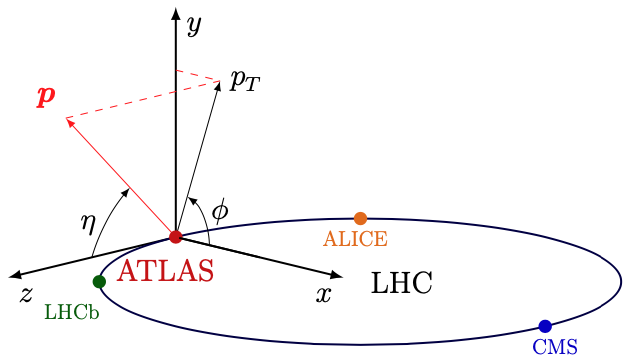
\includegraphics[width=0.6\textwidth]{Images/ATLAS/atlasCoor.png}
  \caption{The ATLAS coordinate system, from \cite{Strong:2020mge}.}
  \label{fig-AtlasCoord}
\end{figure}

As depicted in Figure~\ref{fig-AtlasDec}, ATLAS combines many different systems into one precision machine. These subdetectors are able to measure information in the range $|\eta|<  2.5$, with some specialised subdetectors extending further. An essential component in the detector system are its two types of superconducting magnets. Four central solenoid magnets wrap the point of impact and generate a powerful 2 T magnetic field within the inner detectors along the $z$-axis, while toroidal magnets are placed externally on the barrel and the endcaps muon systems to generate a 3.5 T magnetic field deflecting these leptons in the $\eta$-direction. A $q$-charged particles of momentum $p$ is deflected by a magnetic field $B$ due to the Lorentz force, leading to a connexion between the radius of curvature $R$ of the trajectory and the momentum $p$ such as: 
\begin{equation}
  p_{\perp} = 0.3 \, qBR \, [\text{GeV}/c]
\end{equation}
where $p_{\perp}$ is the magnitude of the momentum perpendicular to the magnetic field $\boldsymbol{B}$, and $q$ is expressed in unit of proton charge. Therefore, from the measurement of the curvature, experimentalists are able to infer the component of the momentum transversial to their generated $B$. Higher magnetic fields lead to larger curvature simplifying the measurement of $R$ and improving the resolution of $p_{\perp}$. \\ 

The rest of this chapter reviews the different subdetectors of ATLAS and introduces some common reconstruction methods that are relevant to the work presented in this thesis. 

\subsection{The Inner Detector Tracker}
The detector placed closest to the point of interaction is the \gls{id} \cite{CERN-LHCC-97-016}. This is a tracker covering the range $|\eta| < 2.5$ in a radius of 3 cm to 1 m, designed to record hits in silicon semiconductors or straw-tubes when charged particles fly through so that their trajectory or \textit{track} can be reconstructed from the collected hits. The powerful 2 T magnetic field of the central solenoids enable this detector to measure both charge and momentum. The \gls{id} combines three subsystems, as represented in Figure \ref{fig-AtlasDecID}. 

\begin{figure}[!h]
  \centering
  \hspace{-1.25cm}
  \makebox[\textwidth][c]{\includegraphics[width=1.1\textwidth]{Images/ATLAS/ATLASinDecComb.png}}
  \caption{The Inner Detector of ATLAS \cite{ATLASschematics}.}
  \label{fig-AtlasDecID}
\end{figure}

First, the high-granularity \textit{Pixel Detector} covers the innermost region with three barrel and three endcap layers, for a total of 80 million sensitive semiconductor-based pixels \cite{CERN-LHCC-97-016, Potamianos:2015lar}. During Run 2, an additional \textit{\gls{ibl}} was added at 33 mm from the centre, with 12 million pixels \cite{Capeans:1291633}. This detector gives robust and precise tracking performance and plays a major role in flavour tagging, as described in Chapter~\ref{chap-ftag}. Pixels are 50 $\mu \times$ 400 $\mu$m in the $R\phi \times z$, with a smaller 50 $\mu \times$ 250 $\mu$m for the \gls{ibl}. The current resolution delivered is of 10 $\mu$m (67 $\mu$m) in the transverse $R\phi$ plane ($z$-direction) \cite{Pernegger_2015, ATL-INDET-PUB-2016-001}. \\

The \textit{\gls{sct}} is the next detector, constructed by arranging pairs of silicon microstrips layers into modules assembled into 4 concentric barrel layers and 9 disks in each endcap \cite{AHMAD200798, CERN-LHCC-2017-005}. The resolution is typically of 17 $\mu$m in $R\phi$ and 580 $\mu$m in $z$ \cite{ATLASSCT}. \\

The final system is the \textit{\gls{trt}}, a gas-based straw-tube tracker aiding track reconstruction by delivering numerous hits \cite{TheATLASTRTcollaboration_2008}. Approximately 300 000 drift tubes of a 4 mm diameter filled with a mélange of argon and xenon are arranged along the beamline in the barrel and radially in the endcaps. Each tube has a conducting wire at its centre and its surface is electrically charged, so that a charged particle flying through ionises the gas, leading to a measurable discharge. Polyethylene is place between the tubes to encourage the emission of transition radiation from relativistic particles proportionally to their Lorentz boost $\gamma ~ E / m$. Consequentely, the \gls{trt} is used both for tracking and electron and pion identification, by reconstructing the mass of the charged particles from the amount of $\gamma$-radiation. For tracking, the position resolution provided is of 130 $\mu$m in the $R\phi$ plane for the barrel and the $z-\phi$ plane in the endcaps \cite{Vogel:1537991}. \\

Altogether, the inverse momentum resolution of the ATLAS \gls{id} is
\begin{equation}
  \sigma(1 / p_T) = 0.36 \oplus \frac{13}{p_T \sin\theta} \text{TeV}^{-1}
\end{equation}
where $\oplus$ is the sum in quadrature \cite{TheATLASCollaboration_2008}. This corresponds to a relative error of 0.01\% for a track with \pt\ $\sim$ 500 MeV, and 4\% at a \pt\ $\sim$ 100 GeV. 

\subsection{Electronic and Hadronic Calorimeters}
Covering the $|\eta| < 4.9$ region, calorimeters collect the energy of all interacting particles, neutral and charged, except for the muons. They are separated into an electromagnetic calorimeter (ECAL) and a hadronic calorimeter (HCAL), each interlaying specific layers of active and passive materials, as displayed in Figure~\ref{fig-AtlasDecCalo}. The passive material typically has a large atomic numbers to induce cascade of particles called \textit{shower}. The active material, tpyically liquid argon (LAr) collects the energy from these showers through ionisation or scintillation light.\\

The ECAL is designed to collect the energy of electrons and photons, as well as contributing to the measurement of the energy of jets. The passive material is lead, with LAr as active material. The ECAL have a depth of 22 $X_0$, where the units of \textit{radiation length} $X_0$ track the distance for an electron to have only 1/$e$ its original energy. The HCAL are designed to capture the energy of hadronic shower, with LAr as active material for the endcap and forward caloriemters and scintillating plastic tiles for the barrel. As passive material, the endcaps use copper plates, the forward calorimeters use copper and tungsten, and the tile calorimeter in the barrel uses steel. The depth of the hadronic calorimeter is $\sim 10 X$, where $X$ is the nuclear interaction length tracking the average distance before a hadron interacts with a nucleus. The calorimeters collect the majority of the energy, with a resolution expressed as
\begin{equation}
  \frac{\sigma_E^{\text{ECAL}}{E} = \frac{10\%}{\sqrt{E}} \oplus \frac{0.7\%}
\end{equation}
for the ECAL, and for the HCAL
\begin{equation}
  \frac{\sigma_E^{\text{HCAL}}{E} = \frac{10\%}{\sqrt{E}} \oplus \frac{0.7\%}.
\end{equation}

\begin{figure}[!h]
  \centering
  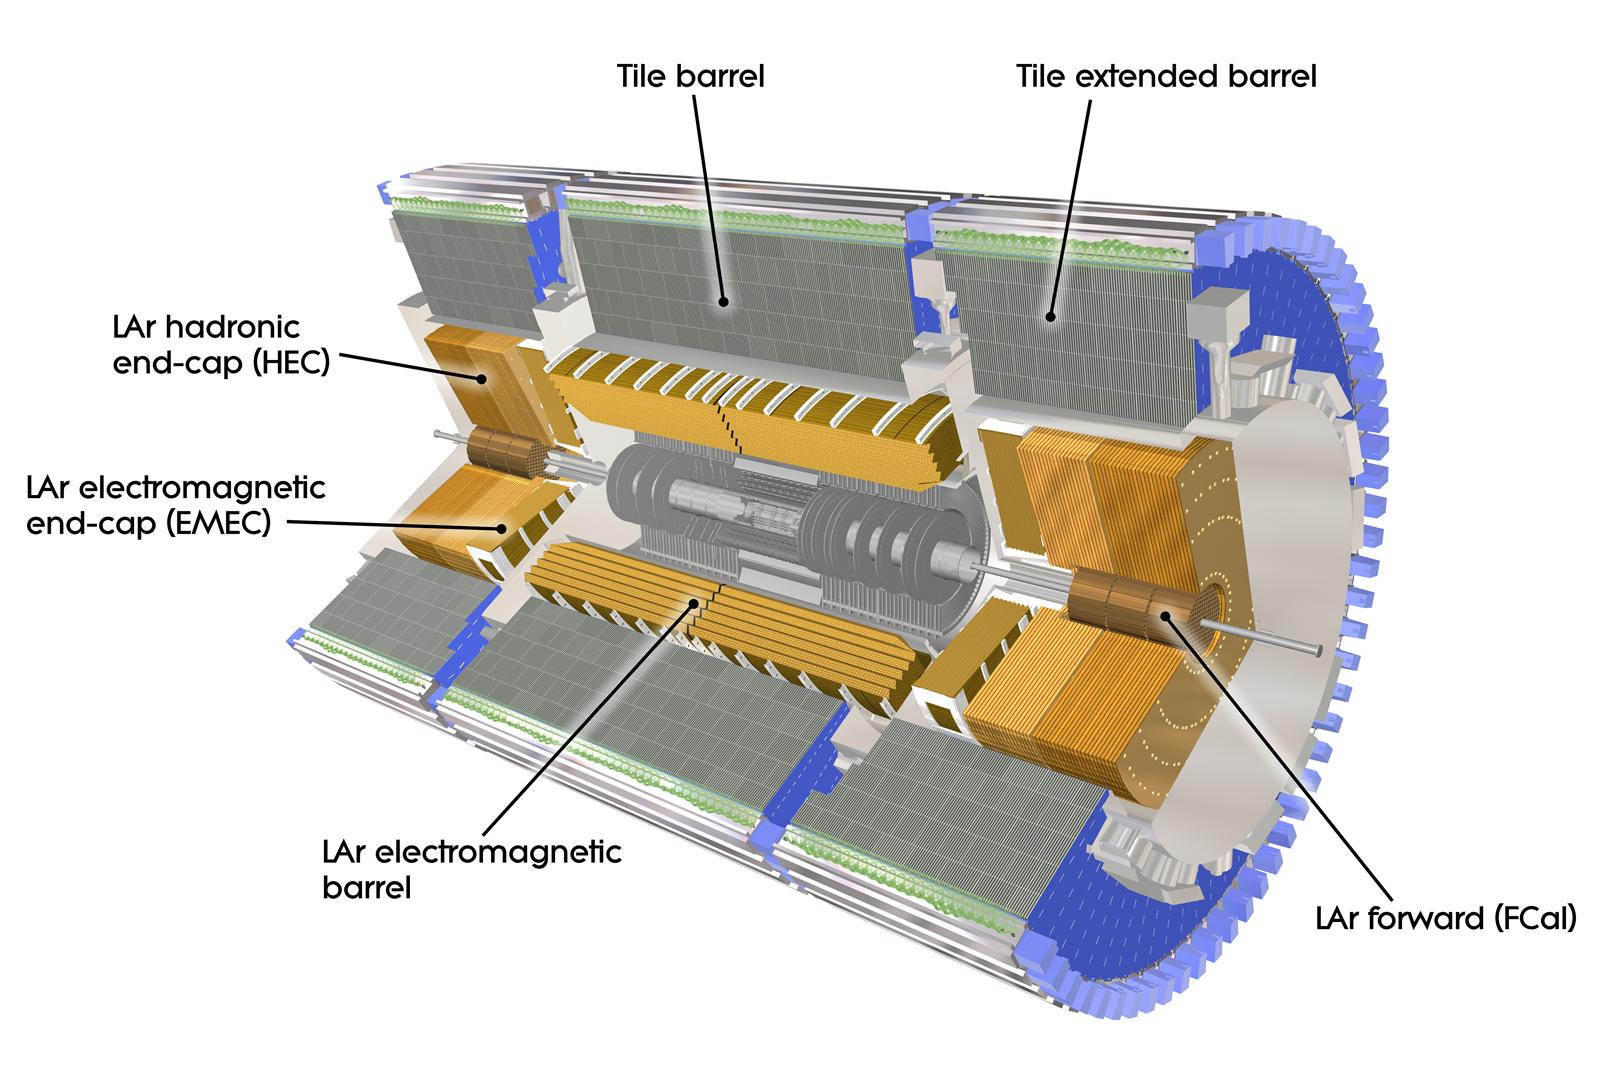
\includegraphics[width=\textwidth]{Images/ATLAS/ATLASCalo.jpg}
  \caption{The calorimeter systems of ATLAS \cite{ATLASschematics}.}
  \label{fig-AtlasDecCalo}
\end{figure}

\subsection{Muon Detection Systems}
\begin{figure}[!h]
  \centering
  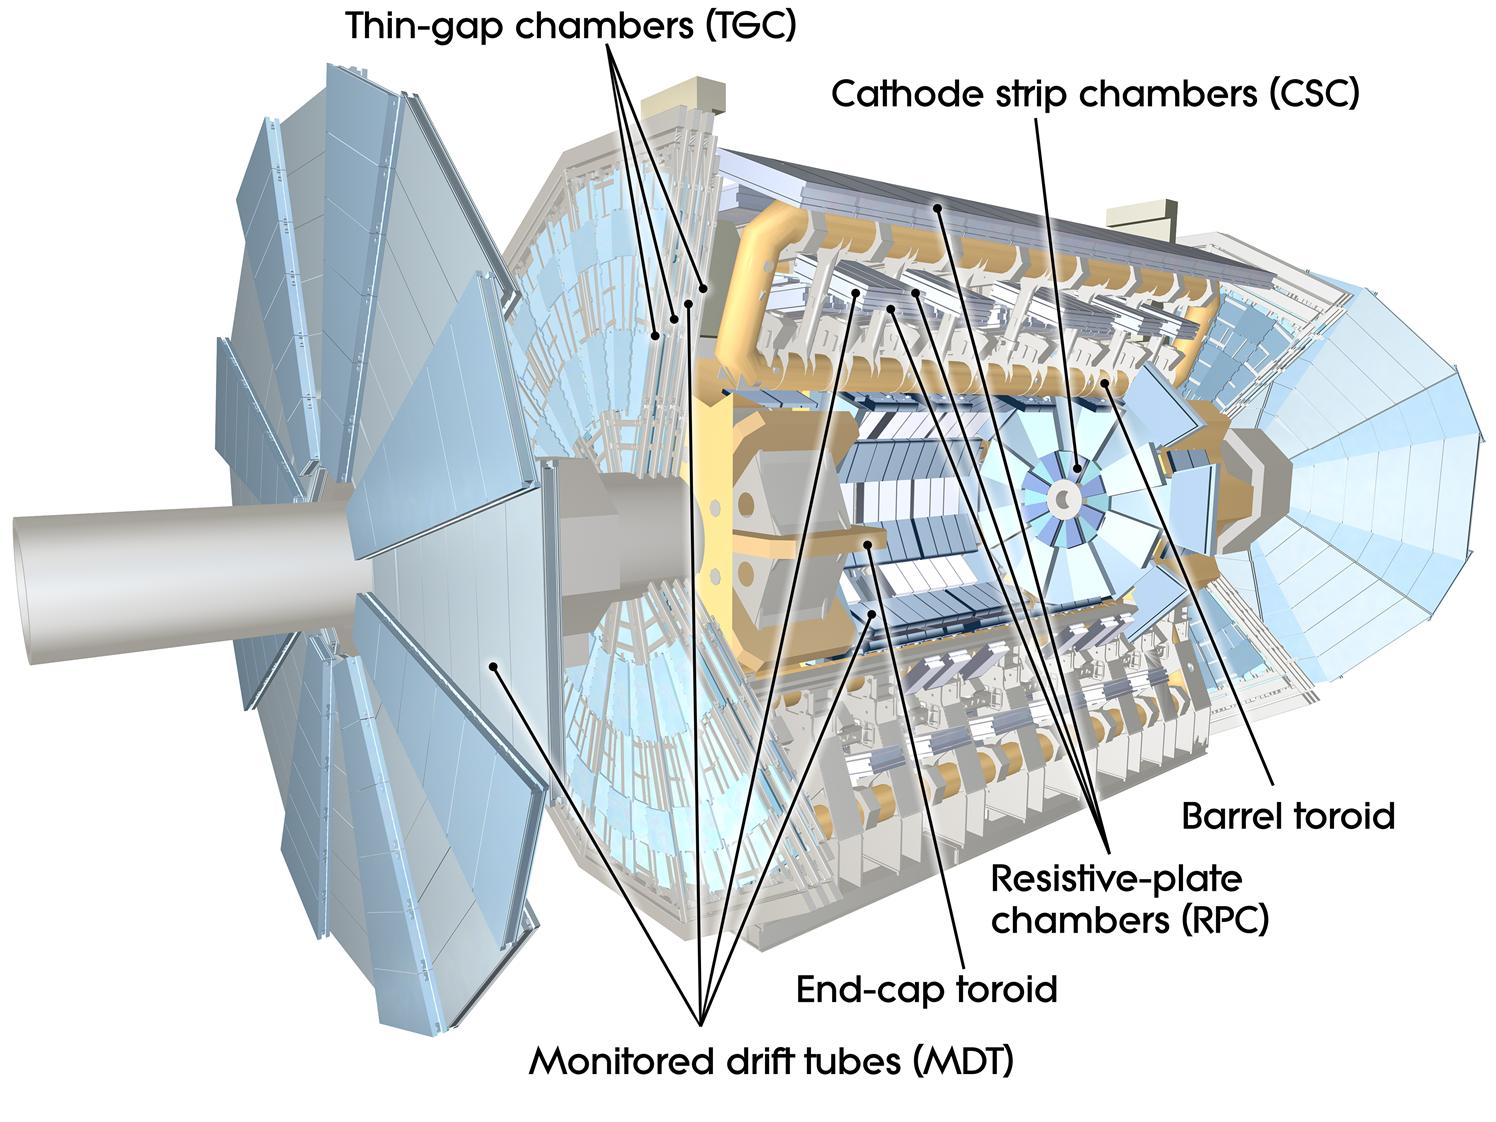
\includegraphics[width=\textwidth]{Images/ATLAS/ATLASMuon.jpg}
  \caption{The muon detectors of ATLAS \cite{ATLASschematics}.}
  \label{fig-AtlasDecMuon}
\end{figure}
